% Imporditud: tools/import_eksperimendid.py
% Allikas: Eesti füüsikaolümpiaadi eksperimendi ülesannete
%   kogu (Rael Kalda, 2023), ülesanne Ü62, lahendus L62.
\setAuthor{EFO žürii}
\setRound{lõppvoor}
\setYear{2013}
\setNumber{P E1}
\setDifficulty{2}
\setTopic{elektriahelad}
\setVahendid{takistitest kolmnurk, patarei, voltmeeter}
\setPunktid{10}
\setAllikas{Eksperimendi kogu Ü62, lahendus lk 60}
\setLahendusseis{toores}

\prob{Kolmnurk}
Kolmest takistist on joonisel kujutatud viisil moodustatud kolmnurk. Leidke
takistite $R_{\mathrm{KR}}$, $R_{\mathrm{RP}}$ ja $R_{\mathrm{PK}}$
takistused, kui on teada, et vähima väärtusega takisti takistus on
$\SI{230}{\ohm}$. Kolmnurga tippudest väljuvad joonisel märgitud värvi
juhtmed.

\begin{center}
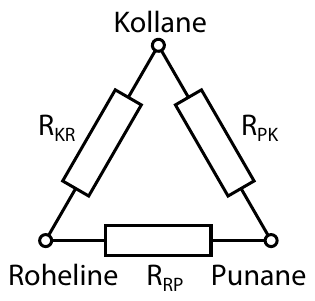
\includegraphics[width=0.25\linewidth]{2013-v3g-pe1-yl.png}
\end{center}

\hint

\solu
Ühendame patarei kahest kolmnurga tipust tulevate juhtmetega (olgu need näiteks

kollane ja roheline). Sel juhul on takistid RRP ja RPK patareiga jadamisi ühendatud

ning mõlemat takistit läbib võrdse tugevusega vool. Mõõdame nendele takistitele

langevad pinged URP ja UP K . Ohmi seaduse järgi kehtib võrdsete voolutugevuste

korral seos RRP = URP . RP K UP K

Seega annab mõõdetud pingete jagatis takistuste RRP ja RP K suhte. Kui kordame samu mõõtmisi veel ülejäänud takistipaaride jaoks, siis saame takistuste suheteks

RP K $\approx$ 2, RRP $\approx$ 2, RRP $\approx$ 4. RKR RP K RKR

Nagu näha, siis on väikseima väärtusega takisti RKR ja ülejäänud takistite takistused on vastavalt RP K $\approx$ 2 $\cdot$ 230 $\Omega$ = 460 $\Omega$ ja RRP $\approx$ 4 $\cdot$ 230 $\Omega$ = 920 $\Omega$.
\probend
